%%=============================================================================
%% Conclusie
%%=============================================================================

\chapter{Conclusie}
\label{ch:conclusie}

% TODO: Trek een duidelijke conclusie, in de vorm van een antwoord op de
% onderzoeksvra(a)g(en). Wat was jouw bijdrage aan het onderzoeksdomein en
% hoe biedt dit meerwaarde aan het vakgebied/doelgroep? 
% Reflecteer kritisch over het resultaat. In Engelse teksten wordt deze sectie
% ``Discussion'' genoemd. Had je deze uitkomst verwacht? Zijn er zaken die nog
% niet duidelijk zijn?
% Heeft het onderzoek geleid tot nieuwe vragen die uitnodigen tot verder 
%onderzoek?

In eerste instantie was het het doel om al een aantal bundlers mogelijks te kunnen schrappen omdat ze zich niet aligneren met de noden van de ontwikkelaars en/of de business binnen Codifly. Hierbij zijn vooral de resultaten van de vragenlijst (Appendix A) van belang (n=9).

\section{Resultaten Vragenlijst Ontwikkelaars}

\begin{figure*}[!htp]
  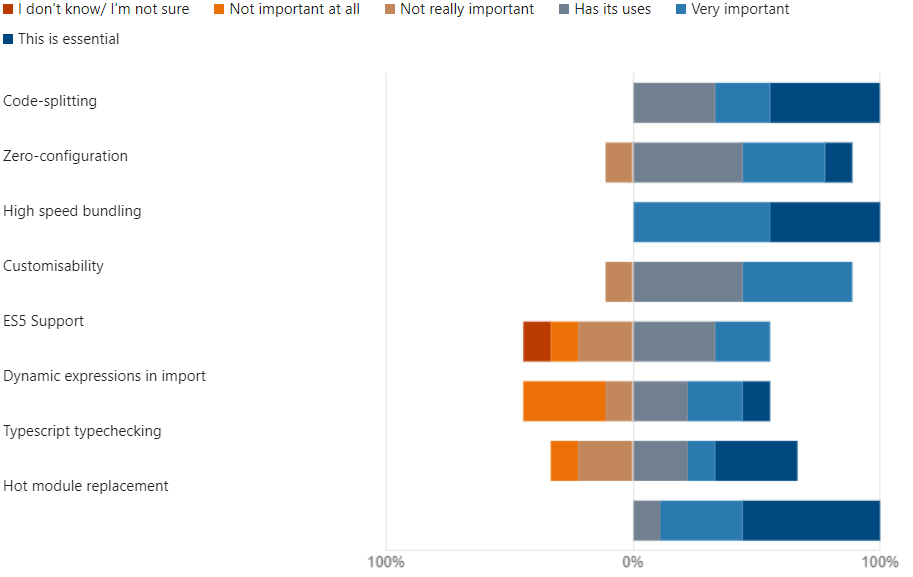
\includegraphics[width=\linewidth]{bachproef/img/graph-developers.png}
  \caption{Overzicht van de antwoorden van developers binnen Codifly op de vragenlijst over bundler features.}
  \label{fig:Devquestionnaire}
\end{figure*}

Grafiek \ref{fig:Devquestionnaire} bevat een overzicht van het sentiment van de ontwikkelaars binnen Codifly naar verschillende features van bundlers:

Uit bovenstaande grafiek vallen de volgende conclusies gemaakt te worden:

\begin{itemize}
    \item ``Code-splitting'', ``high speed bundling'' en ``hot module replacement'' zijn universeel positief bekeken.
    \item ES5-ondersteuning ligt lager op de lijst van prioriteiten, hoewel er enige onzekerheid overblijft.
    \item ``Dynamic expressions in import'' en TypeScript typechecking hebben verdeelde antwoorden.
    \item Zero-configuration wordt door de meerderheid als positief bekeken.
\end{itemize}

Dit heeft als gevolg op de bundlers dat ESBuild en Rollup buiten de gewenste categorie vallen. ESBuild heeft onder andere slechts work-in-progress ondersteuning voor code-splitting. Anderzijds is Rollup vooral gefocust op productie-builds en optimalisatie van de bundels, wat resulteerd in weinig tot geen voordeel in een ontwikkelingsomgeving.

\section{De Noden van de Business}

Hoe sluiten de noden van de business hiermee aan? Aangezien ESBuild tot op heden toe nog niet een v1.0 release heeft, maakt dit het ook geen aantrekkelijke optie om mee van slag te gaan. Rollup voldoet hier wel aan, maar is ook hevig op configuratie en is als gevolg op zichzelf ook niet een ideale keuze om mee aan de slag te gaan.

\section{Resultaten Benchmarks}

In deze sectie zal per project dichter gekeken worden naar de resultaten van de benchmarks, startende met de website van Codifly zelf. De volledige resultaten zijn beschikbaar in bijlage \ref{appendix:benchmarks}.

\subsection{De Corporate Website}

\begin{figure*}[!htp]
  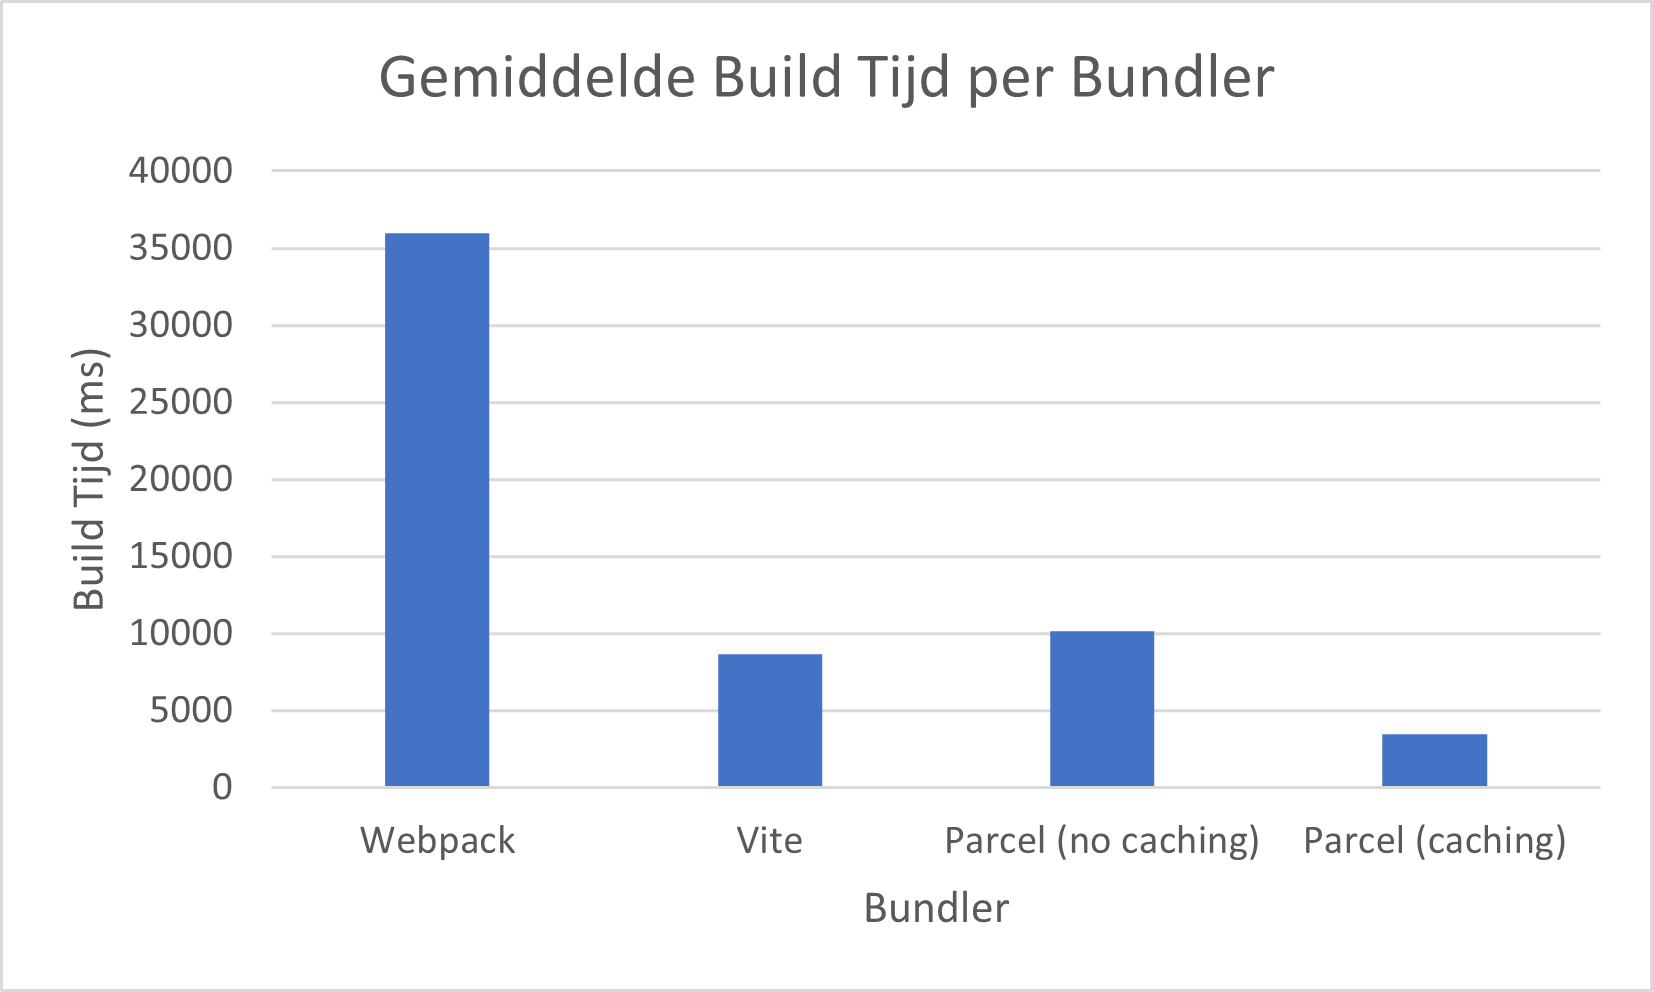
\includegraphics[width=\linewidth]{bachproef/img/results-corporate.png}
  \caption{Staafgrafiek van de gemiddelde tijd om de devserver van bundlers op te starten voor de corporate website van Codifly.}
  \label{fig:Corporateresults}
\end{figure*}

\begin{figure*}[!htp]
  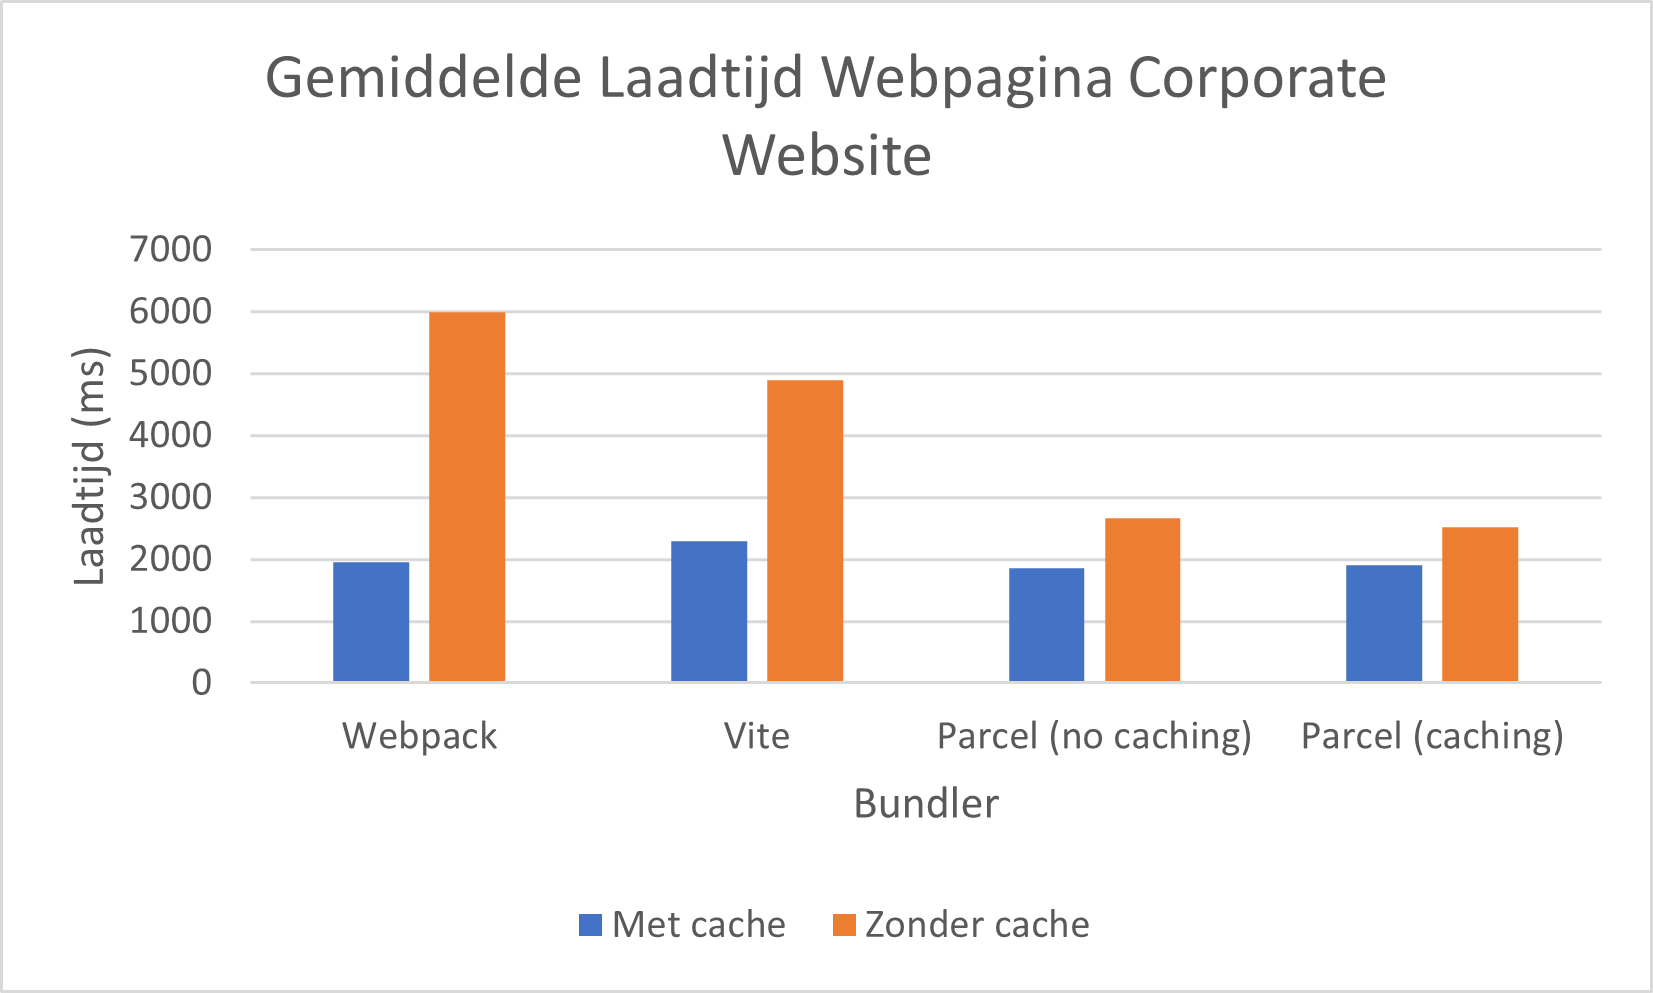
\includegraphics[width=\linewidth]{bachproef/img/results-corporate-load.png}
  \caption{Staafgrafiek van de gemiddelde tijd om de pagina te herladen voor de corporate website van Codifly.}
  \label{fig:Corporateresultsloadtimes}
\end{figure*}

In grafiek \ref{fig:Corporateresults} wordt de gemeten tijd van de tijd om de devserver op te starten gevisualiseerd:

Zoals verwacht, maakt het gebruikt van natively compiled code een zeer groot verschil op de bundeltijden. Webpack wordt met een gemiddelde tijd van 36 seconden overtroffen door beide Parcel en Vite. Tussen Parcel en Vite is de vergelijking moeilijker. Op eerste zicht heeft Parcel gewonnen puur afgaand van tijd, maar er zijn ook nog andere aandachtspunten. De onderzoeker heeft bijvoorbeeld ondervonden dat de configuratie makkelijker verliep met Vite dan met Parcel. Met de huidige indeling van dit project was het de onderzoeker niet gelukt om binnen een redelijke tijd ervoor te zorgen dan de videobestanden ook bijgevoegd werden in de development server. Belangrijk om op te merken is dan ook dat dit enig effect kan gehad hebben op de cijfers van Parcel, hoewel dit waarschijnlijk vooral zo zou zijn geweest bij de cijfers zonder caching. Bij de configuratie van Vite werd ook wat dubbel werk nodig, want dat de configuratie werkt voor de development server betekent niet dat die ook werkt voor de productie-builds die met Rollup gemaakt worden. In de ervaring van de onderzoeker viel dit echter goed mee, en was een volledig functioneel resultaat bemachtigd.

Een gelijkaardig patroon doet zich voort in grafiek \ref{fig:Corporateresultsloadtimes}. Hier is er echter een zeer duidelijke winnaar bij het herladen zonder cache. De onderzoeker vermoedt dat dit een testament is van de zeer efficiënte caching-strategie die Parcel toepast.
Met cache is de tijd echter heel gelijkaardig. De onderzoeker vermoedt dat Vite hier verliest door de no-bundler aanpak, waardoor de browser meer moeite moet vergaren om de pagina te laden.

\subsection{Het Seed-project}

\begin{figure*}[!htp]
  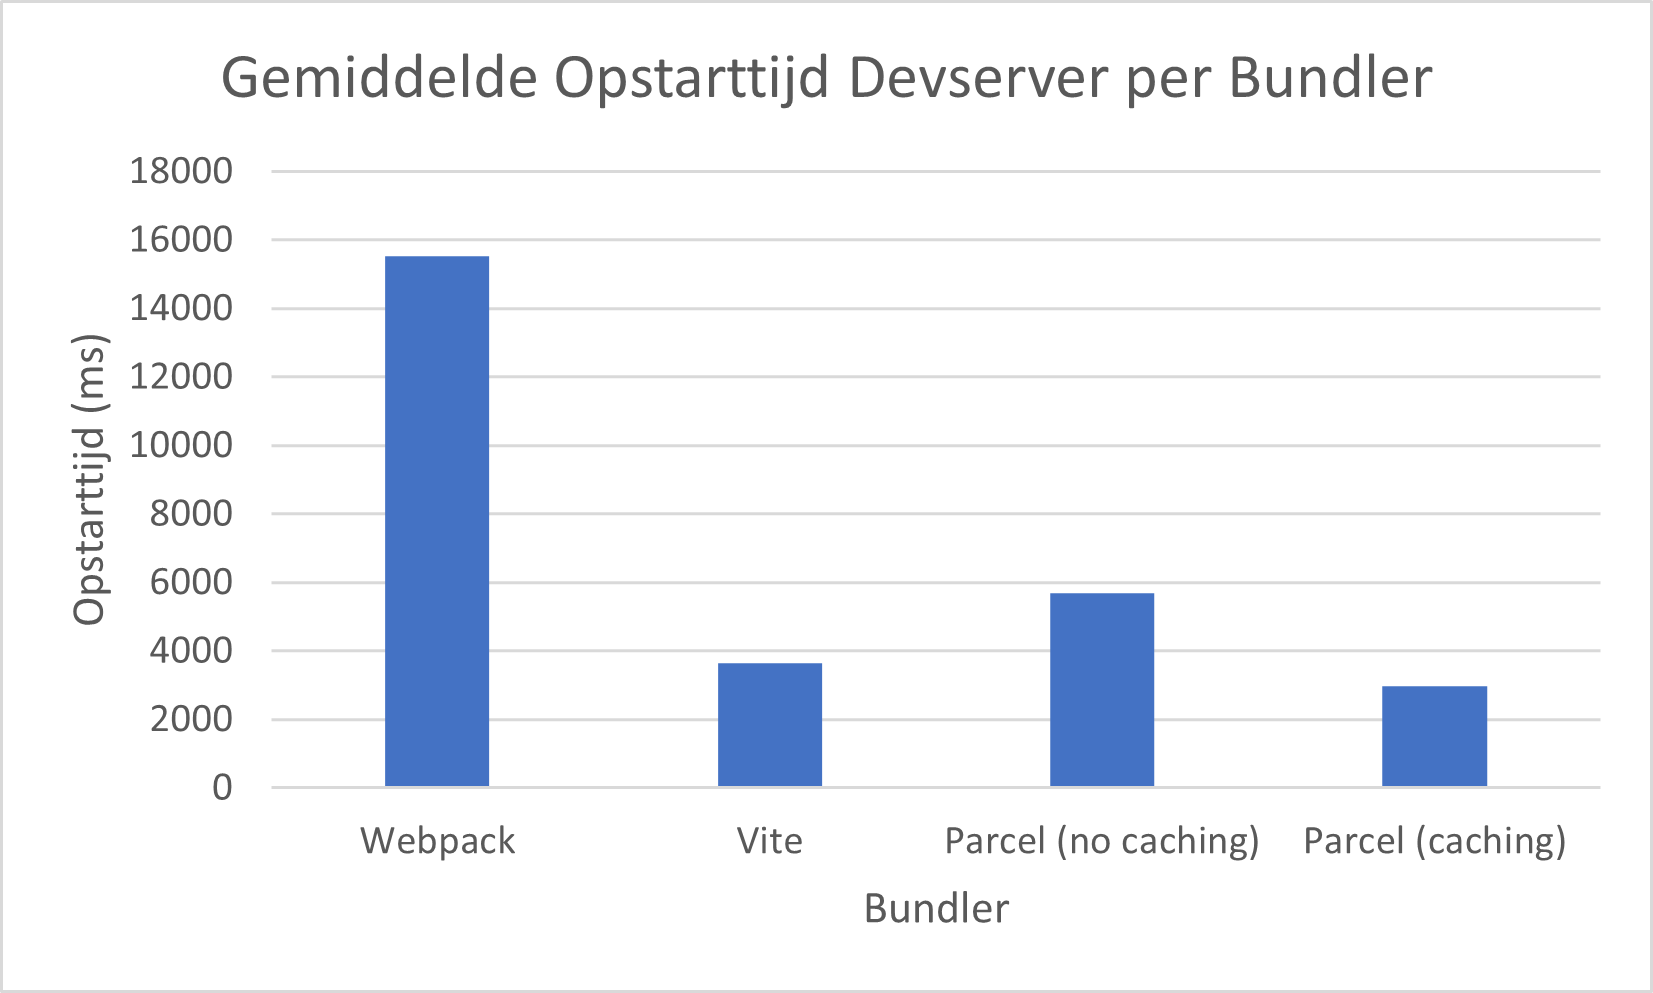
\includegraphics[width=\linewidth]{bachproef/img/results-seed.png}
  \caption{Staafgrafiek van de gemiddelde tijd om de devserver van bundlers op te starten voor het seed-project van Codifly.}
  \label{fig:Seedresults}
\end{figure*}

\begin{figure*}[!htp]
  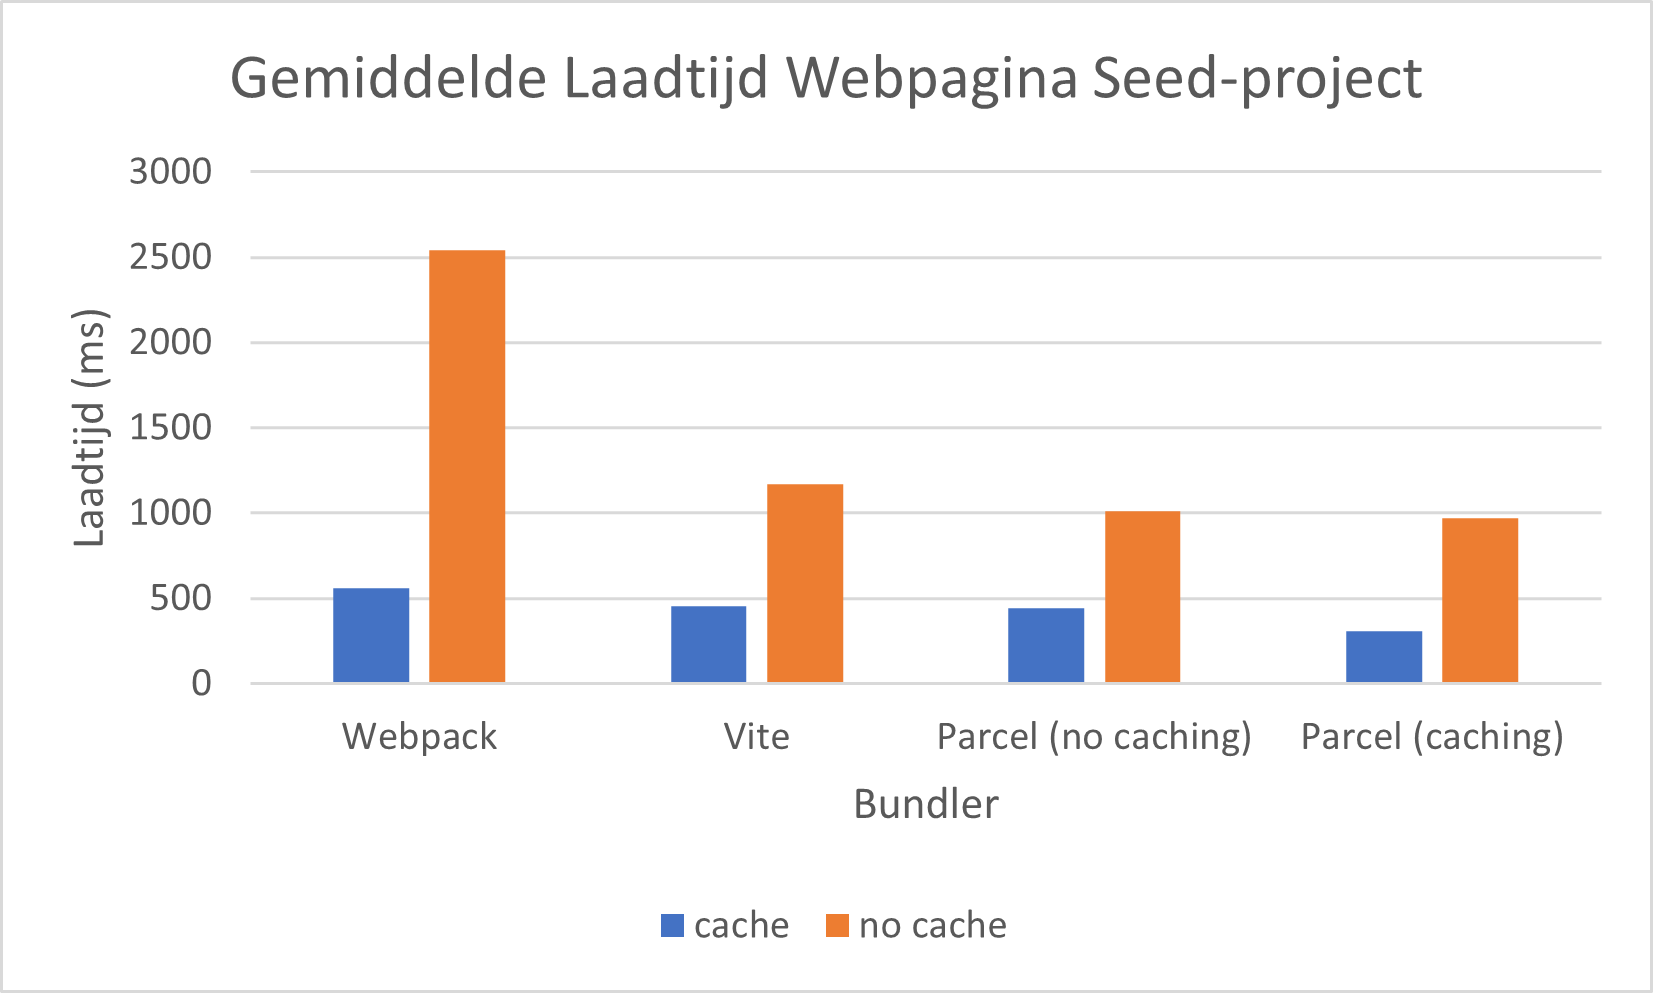
\includegraphics[width=\linewidth]{bachproef/img/results-seed-load.png}
  \caption{Staafgrafiek van de gemiddelde tijd om de pagina te herladen voor het seed-project van Codifly.}
  \label{fig:Seedresultsloadtimes}
\end{figure*}

Zoals te zien in grafiek \ref{fig:Seedresults} is de trend van de resultaten in dit project gelijkaardig aan die bij de corporate website. Webpack bewijst alweer de traagste te zijn met een gemiddelde opstarttijd van 15,5 seconden. Parcel en Vite zijn daarentegen nek aan nek, met Parcel die de kroon neemt bij het gebruik van caching.

Uit grafiek \ref{fig:Seedresultsloadtimes} kunnen ook gelijkaardige conclusies gemaakt worden als bij de corporate website. Hier is de tijd van Vite echter plots zeer gelijkaardig aan die van Parcel. Dit is mogelijks te verklaren door het feit dat er minder modules ingeladen moeten worden in dit project, wat ook de gelijkaardige laadtijden met caching zou verklaren.

\subsection{Algemene Observaties en Opmerkingen}

Naast de testresultaten zelf, zijn er nog andere observaties die gemaakt werden door de onderzoeker tijdens het migreren van de projecten naar de nieuwe bundlers. Onder andere zijn de volgende observaties gemaakt:

\begin{itemize}
    \item Vite heeft gelijkaardige configuratie-opties aan Webpack, dit maakt het overstappen van Webpack naar Vite gemakkelijker.
    \item De configuratie van Vite kan in TypeScript gemaakt worden, Parcel doet dit met een .parcelrc bestand in een json-syntax. Het is echter gemakkelijker om te werken met configuratie in Typescript, en ook de huidige strategie bij de Webpack configuratie van Codifly-projecten.
    \item Vite heeft een betere ondersteuning en groter aanbod aan community plugins.
    \item Doordat Vite niet dezelfde bundler gebruikt voor development- en productie-builds moet er gelet worden op of alles goed werkt in een productie-build. Dit kan met het preview-commando dat lokaal een productie-build draait.
    \item De Webpack-versie van de corporate website is 4 en wanneer vergeleken met de v5 builds in het seed-project is v5 toch al veel performanter dan v4.
\end{itemize}
